\section{Síťový analyzátor Wireshark}\label{wireshark}
Wireshark je grafická aplikace sloužící k zachytávání paketů a jejich analýze, viz obrázek \ref{fig:wireshark-layout}. Wireshark umí zachytávat provoz na lokálních fyzických či virtuálních síťových rozhraních počítače. Alternativou ke grafickému Wireshark je řádkový nástroj \texttt{tcpdump}. 

\begin{figure}[h]
  \centering
  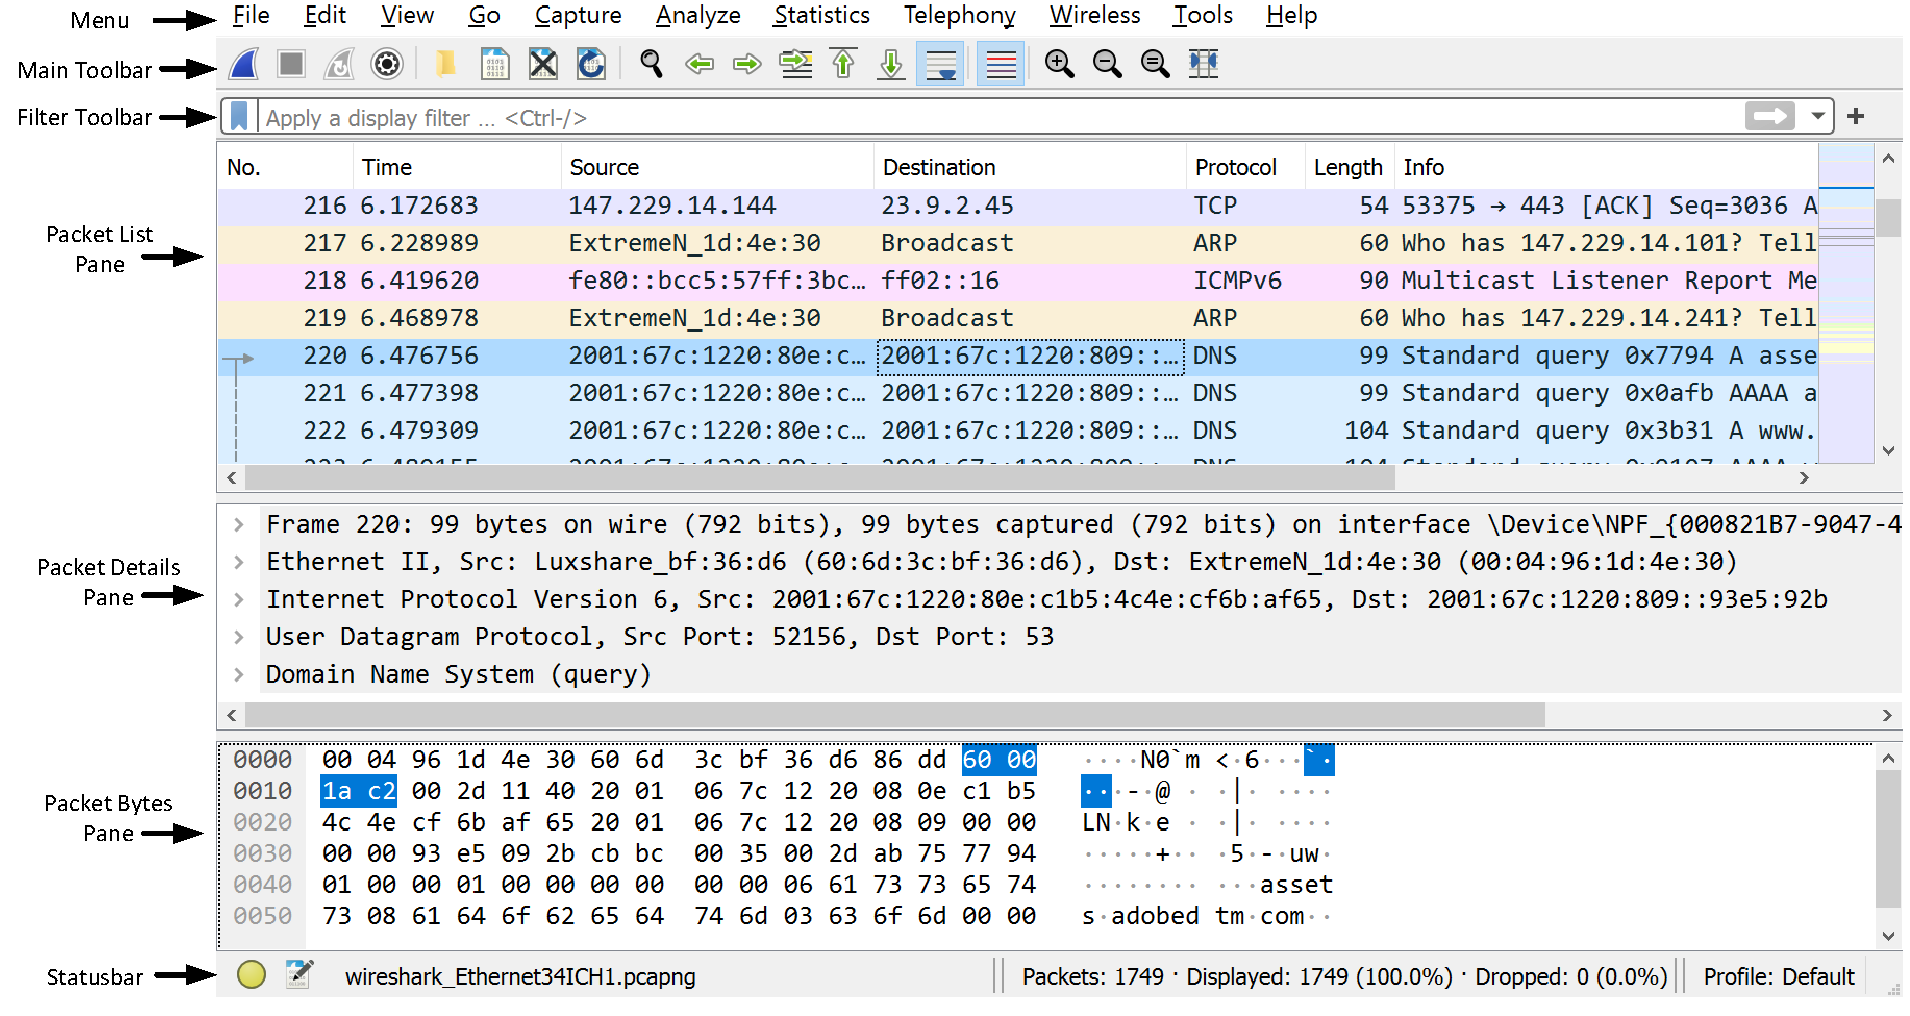
\includegraphics[width=170mm]{fig/wireshark-layout.pdf}
  \caption{Wireshark}\label{fig:wireshark-layout}
\end{figure}

\subsection{Zachytávání provozu (Packet Capturing)}
Následující kroky popisují zahájení zachytávání paketů v programu Wireshark:
\begin{enumerate}
  \item Zachytávat provoz můžeme z vybraného síťového rozhraní nebo z~více rozhraní najednou. Rozhraní můžeme vybrat v menu \texttt{Capture -> Options}.
  \item V nastavení je také možné nastavit filtr pro zachytávání paketů (Capture Filter), který sníží počet zpracovaných a zobrazených paketů. Políčko {\tt Capture Filter} umožňuje vybrat již předdefinovaný filtr nebo je možné si vytvořit vlastní filtr, viz {\tt man pcap-filter}.
  \item Záchyt spustíme pomocí tlačítka \texttt{Start}.
  \item Odchycený provoz (pakety spolu s časovými značkami)  můžeme uložit do souboru typu PCAP. Později je možné zachycený provoz analyzovat.
\end{enumerate}

\subsection{Výběr zachyceného provozu pomocí zobrazovacího filtru (Display Filter)}
Často je vhodné zobrazit pouze část zachyceného provozu, který nás zajímá, např. komunikaci HTTP. K tomu můžeme využít zobrazovací filtr (Display Filter), který se nachází pod nástrojovou lištou. Syntax filteru je popsána v tabulce \ref{tab:display-filter}. 

\begin{center}
  \begin{table}[h]
    \centering
    \def\arraystretch{1.2}
    \begin{tabular}{|l|l|}
      \hline
      \textbf{Porovnávání} & \texttt{==, >=, <=, !=, contains}\\
      \textbf{Logické operátory} & \texttt{||, or, \&\&, and, !, not}\\
      \textbf{Kombinace filtrů} & \texttt{(ip.src==192.168.0.105 and udp.port==53)}\\
      \textbf{Filtrování na základě existence pole} & \texttt{http.cookie or http.set\_cookie}\\
      \textbf{Filtrování specifických bytů} & \texttt{eth.src[4:2]==22:1b}\\
      \textbf{Regex filtrování} & \texttt{http.host \&\& !http.host matches "\.com\$"}\\
      \hline
    \end{tabular}
    \caption{Filtrovací operátory}\label{tab:display-filter}
  \end{table}
\end{center}

\subsection{Zobrazení toků (Flow Graph)}
Wireshark umožňuje zobrazit časovou posloupnost komunikace pomocí tzv. grafu toků \texttt{flow graph}, viz \texttt{Statistics -> Flow Graph..}. Graf toků zobrazuje komunikaci mezi jednotlivými zařízeními definovanými IP adresou. Je zde vidět, jak často spolu stanice komunikují, jaké zpráva a v jakém pořadí posílají. 

\subsection{Zobrazení obsahu toku (Stream Analysis)}
Wireshark zachytává jednotlivé pakety. Pokud chceme vidět obsah celé komunikace, např. HTTP můžeme pro zobrazení komunikace (streamu) použít volbu \texttt{Flow <protokol> Stream}. Zobrazení toku provedeme tak, že vybereme jeden zachycený paket, klikneme na něj pravým tlačítkem myši a vybere volbu  \texttt{Follow <protokol> Stream}.

\subsection{Časové značky}
Každý paket obsahuje časovou značku svého záchytu. Zobrazení časové značky závisí na nastavení Wiresharku. Wireshark umožňuje zobrazit čas jako časovou značku obsahující datum a čas záchytu, absolutní čas, relativní čas od záchytu komunikace a další. Formát času můžeme nastavit v menu \texttt{View -> Time Display Format}.
